\chapter{Microservices Architecture}

This chapter looks at \textbf{Microservices Architectures}, covering the basic ideas, principles, and benefits that make it popular in modern software development. First, let’s answer an important question: How do we break a system into \textit{components}?

Breaking a system into components is a key step in adopting Microservices Architectures. Here are some reasons for doing this: it allows different teams to work in parallel, promotes reusability, makes it easier to distribute systems across multiple computers, and supports smooth replication, parallel execution, and migration to take full advantage of cloud capabilities like scalability, reliability, and flexibility.

As we explore the main principles of Microservices Architectures, we highlight the importance of stateless services that store \textit{persistent information in local databases}. This approach helps ensure agility and scalability, allowing services to move between virtual servers as needed, while also helping to create resilient and fault-tolerant systems. \\

Software components that can be accessed over the Internet are called \textbf{software services}. A service is accessed through its \textit{published interface}, where all implementation details are hidden. Given an input, a service produces a corresponding output without side effects. Services \textit{do not maintain any internal state} because state information is either stored in an explicit database or maintained by the service requestor. Interactions where the state is maintained involve service requests that have the state and the service result integrated with the answer to the request. \\

\noindent Some history that led to microservices architectures:

\begin{itemize}
    \item \textbf{Service-oriented architecture} (\textbf{SOA}, late 1990s): applications made up of many blocks, where each block is a class or an object. Those (\textit{independent}) blocks could have been written in different technologies since they communicated with each other (or the Internet) through public interfaces.
    \newpage
    \item \textbf{Web Services} (early 2000s): services were standard-based (XML, SOAP, WSDL, and many others), where the standards were used to describe the services (input, output, type of parameters, and so on). Standards were good, but having many standards made them hard to handle.
    \item \textbf{Modern service-oriented systems} (nowadays): much simpler interaction protocols, much simpler interfaces (with more efficient formats for encoding message data), which led to lower overhead and faster execution.
\end{itemize}

Amazon Web Services\footnote{\url{https://aws.amazon.com/}} had a significant impact on this service world, providing a manifesto with guidelines on \textbf{how services should be implemented}: a service should be related to a \textit{single business function}; services should be completely \textit{independent}, with their \textit{own databases}; a service should manage its own user interface; it should be possible to replace/replicate a service without changing other services. This leads to \textbf{microservices}: generally small-scale stateless services that have a single responsibility.

\begin{figure} [H]
    \centering
    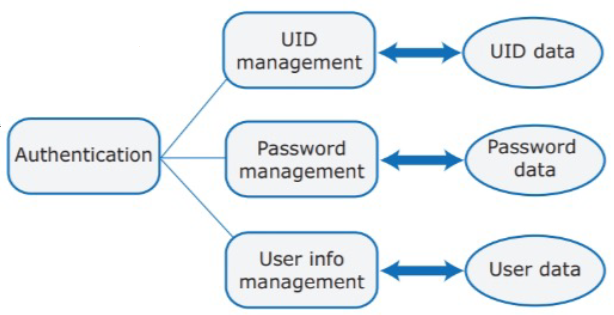
\includegraphics[width=0.7\textwidth]{images/Microservices/service_example.png}
    \caption{Example of a system using an authentication module}
    \label{fig:service_example}
\end{figure} 

Taking a system that uses an authentication module (providing user registration, authentication using UID/password, two-factor authentication, user information management, password reset), we can see from Figure \ref{fig:service_example} an example of a segmentation into microservices. In order to \textit{identify the microservices} that might be used for the authentication system, developers need to break coarse-grained features into more detailed functions, look at the data used, and identify a microservice for each logical data item to be managed (each service will have its own data). In the case that one service needs the data of another service, it can request it through interfaces or just replicate some critical data (facing consistency), minimizing the amount of replicated data management.

\subsection{Microservices}

We have already defined microservices as \textit{independent} (service interfaces not affected by changes to other services) and (generally) small-scale services that can be combined to create applications. It must be possible to modify and redeploy a service without changing/stopping other services.
\newline\noindent
Some of the characteristics that microservices must have are:

\begin{itemize}
    \item \textbf{Self-contained}: Microservices do not have too many external dependencies. They manage their own data and implement their own user interfaces. This allows them to deploy and change the applications immediately.
    \item \textbf{Lightweight}: Microservices communicate using lightweight protocols so that the service communication overhead is low.
    \item \textbf{Implementation independent}: Microservices may be implemented using different programming languages and may use different technologies in their implementation.
    \item \textbf{Implementation deployable}: Each microservice runs in its own process and is independently deployable using automated systems.
    \item \textbf{Business-oriented}: Microservices should implement business capabilities and needs rather than simply provide a technical service. This characteristic coincides with Agile frameworks.
\end{itemize}

Two of the measures used for microservices are \textbf{coupling} (which measures the number of inter-component relationships) and \textbf{cohesion} (which measures the number of intra-component relationships). Developers should achieve \textit{low coupling} and \textit{high cohesion}: \textit{low coupling} means independent services and independent updates, while \textit{high cohesion} means less inter-service communication overhead. \\

Each service should do one thing only, and it should do it well (\textbf{Single Responsibility Principle}). In order to understand \textit{how big a microservice should be}, we can use \textit{the rule of twos}: a service can be developed, tested, and deployed by a team in two weeks. The team can be fed with two large pizzas (8-10 people). 

This amount of people is required because they have to implement service functionality, develop code that makes the service completely independent, process incoming and outgoing messages, manage failures (there will most likely be service and interaction failures), manage data consistency (which becomes severe in the case of data replication) when data are used by other services, maintain the service's own interface, test the service and service interactions, and support the service after deployment (you build it, you run it). Years ago, there were different teams for development and production stages, but now DevOps (the same people who build and maintain the service) is widely used.

\section{Architecture}

The main motivations behind the need for microservices architectures are \textit{shortening lead time for new features and updates} and \textit{scaling}. Deploying microservices in separate containers allows for quickly stopping and restarting the microservice without affecting the other services, and replicas can be quickly deployed. If these two reasons are important for the application, then microservices are the way to go; otherwise (in the case of a simple application), a monolithic application will work just fine.

\begin{figure} [H]
    \centering
    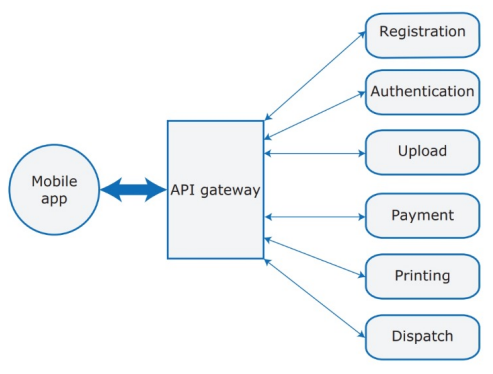
\includegraphics[width=0.65\textwidth]{images/Microservices/photo-printing-system.PNG}
    \caption{Photo-printing system for mobile devices}
    \label{fig:photo-printing-system}
\end{figure} 

From Figure \ref{fig:photo-printing-system}, it's possible to understand that microservices allow us to identify the basic services of an application, as we have separated services for each area of functionality. It also shows that it's good practice to use an \textbf{API gateway} to provide a single point of contact from the mobile application to the microservices. It will be the gateway's job to redirect requests to the appropriate microservice.\\
\newline \noindent
There are five different \textbf{architectural design decisions} that need to be addressed when it comes to microservices architectures:

\begin{enumerate}
    \item What are the microservices that make up the system?
    \item How should microservices communicate with each other?
    \item How should data be distributed and shared?
    \item How should the microservices in the system be coordinated?
    \item How should service failure be detected, reported, and managed?
\end{enumerate}

\noindent These points will be developed throughout the rest of the section.

\subsection{System Decomposition}

The \textbf{system decomposition} is one of the most important design choices, but it is also not an easy task. Having too many microservices will lead to \textit{low cohesion} (which means a lot of communication overhead), while having too few will lead to \textit{high coupling} (which means less independence for updates, deployment, and so on).\\
\newline \noindent Some tips are:
\begin{itemize}
    \item Find the right balance between fine-grained functionality and system performance.
    \item Follow the \textit{common closure principle} (elements likely to be changed at the same time should stay in the same service).
    \item Associate services with business capabilities.
    \item Services should have access only to the data they need (with some data propagation mechanisms).
\end{itemize}

It's usually hard to think in terms of microservices; that's why it's common to start with a monolith and decompose it later. One way to understand how microservices should be split is to look at the data services have to manage.

\subsection{Service Communications}

Another design choice is how the services communicate.

\begin{figure} [H]
    \centering
    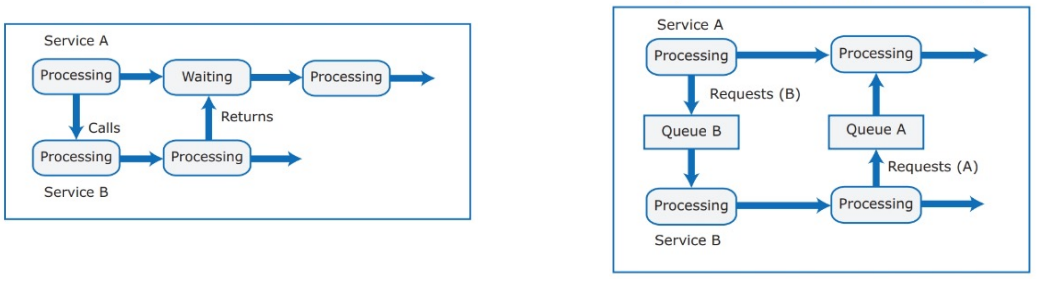
\includegraphics[width=1\textwidth]{images/Microservices/sync-vs-async.PNG}
    \caption{Synchronous vs. asynchronous service interaction}
    \label{fig:sync-vs-async}
\end{figure} 

As shown in Figure \ref{fig:sync-vs-async}, one choice is to go for \textbf{synchronous} or for \textbf{asynchronous} communication: the first one (which in the Figure is the one on the left) is easier to write and understand, while the second one (which in the Figure is the one on the right) has low coupling, is more efficient, but is more difficult to write (since a queue for the requests is required) and to understand.

\begin{figure} [H]
    \centering
    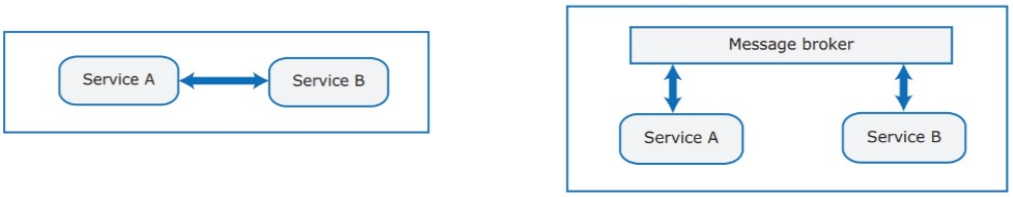
\includegraphics[width=1\textwidth]{images/Microservices/direct-vs-ind.PNG}
    \caption{Direct vs. indirect service communication}
    \label{fig:direct-vs-ind}
\end{figure} 

The second choice is to either choose \textbf{direct} or \textbf{indirect} service communication: the first one consists of allowing one service to send messages directly to another service (it's simpler and faster, but the requester must know the other services' URIs), while the second one utilizes a message broker or a queue that finds the address of the requested service and handles the message translation. The indirect communication supports both synchronous and asynchronous interactions; it is easier to modify and replace services, but it is more complex and slower.

\subsection{Data Distribution and Sharing}

Each microservice should \textbf{manage its own data}, as we want to achieve independence between microservices (so other microservices shouldn't know how data is organized). There will be data dependencies between microservices, and some of the ways to deal with them are:
\begin{itemize}
    \item Data sharing should be as minimal as possible.
    \item Sharing should be read-only, with a few services responsible for data updates.
    \item Include a mechanism to keep database copies used by replicated services consistent.
\end{itemize}

One mechanism to keep database copies consistent is \textbf{ACID}\footnote{ACID: Atomicity, Consistency, Isolation, Durability} \textbf{transactions}, where updates are serialized (which means that the database moves from one consistent state to another) to avoid inconsistency. While in distributed systems we must trade off data consistency and performance, with microservices systems, developers must design the system to \textit{tolerate some degree of data inconsistency}. Two types of data inconsistency that must be managed are:
\begin{itemize}
    \item \textbf{Dependent data inconsistency}: Actions or failures of one service can cause data managed by another service to become inconsistent.
    \item \textbf{Replica inconsistency}: Several replicas of the same service may be executing concurrently, each with its own database copy, and each updating its own database copy (so those databases should be \textit{eventually}\footnote{eventually: sooner or later} \textit{consistent}).
\end{itemize}

\subsubsection{CAP Theorem}

Brewer’s conjecture (PDOC 2000) states that: ``\textit{it is impossible for a web service to provide \textcolor{red}{C}onsistency, \textcolor{red}{A}vailability, and \textcolor{red}{P}artition tolerance at the same time}'', where \textit{\textcolor{red}{C}onsistency} means that each service returns the correct response to each request, \textit{\textcolor{red}{A}vailability} means that each request eventually receives a response, and \newline \textit{\textcolor{red}{P}artition tolerance} means that services can be partitioned into multiple groups, and the network can delay or lose arbitrarily many messages among services. \\

A later reformulation (made in 2012 by Gilbert \& Lynch) states that: \textit{In a network subject to communication failures, it is impossible for any web service to implement an atomic read/write shared memory that guarantees a response to every request} (which implies that you must choose between \textit{consistency} and \textit{availability}). \newline
A simple proof sketch is: Let S1 and S2 be two services belonging to two different network partitions, where every message from S1 to S2 may be delayed or lost. Since S2 can't always be sure whether S1 received the write request or not (because the confirmation from S1 to S2 may be delayed or lost), in the case that S2 sends two different write requests with values V1 and V2, S2 cannot distinguish between the following two cases: S1 received a write request of value V1 and sent an OK response; or S1 received a write request of value V2 and sent an OK response. This leads to a state in S2 that cannot determine whether to return V1 or V2 in response to a read request (because S2 should reply with the same value that S1 does).

\noindent Some practical solutions are:
\begin{itemize}
    \item Guarantee availability and provide best-effort consistency (general solution).
    \item Guarantee strong consistency and provide best-effort availability (this solution is implemented when strong consistency is required (e.g financial applications)).
    \item Trade off consistency and availability (e.g., tolerate being one hour out of date but not one day out of date).
\end{itemize}

\subsubsection{The Saga Pattern}

\begin{wrapfigure}{r}{0.18\textwidth}
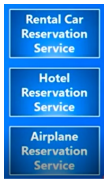
\includegraphics[width=0.18\textwidth]{images/Microservices/Saga.PNG}
    \caption{Saga example}
    \label{fig:Saga}
\end{wrapfigure}

How can we implement distributed transactions with a pattern? \textbf{The Saga pattern} consists of implementing each business transaction that spans multiple services as a \textit{saga}, where a \textit{saga} is a sequence of local transactions (see Figure \ref{fig:Saga}). Each local transaction updates a database and triggers the next local transaction(s) in the saga. If a local transaction fails, then the saga executes a series of compensating transactions (instead of rolling back, since in microservices sometimes rolling back isn't possible).

There are two ways of coordinating sagas: \newline\textbf{Choreography}, where each local transaction publishes events that triggers the next local transaction(s); or \textbf{Orchestration}, where an \newline orchestrator tells participants which local transactions to execute.

There are again two ways of compensating transactions: \newline\textbf{Backward model}, where changes made by previously executed local transactions are undone; and \textbf{Forward model}, where the “retry later” principle is applied. \\

The \textit{Netflix approach} consists of the replication of data in n nodes using \textit{Apache Cassandra}\footnote{\url{https://cassandra.apache.org/_/index.html}} to achieve eventual consistency: the system tries to update as much as possible, ensuring that at least (n/2 + 1) of the replicas must respond. This is one example of a compromise that can be achieved with eventual consistency.

\subsection{Service Coordination}

There are two possible ways to implement \textbf{service coordination}: 
\begin{itemize}
    \item \textbf{Orchestration}, where an orchestrator tells the microservices how they should “play”.
    \item \textbf{Choreography}, where microservices manage themselves.
\end{itemize}
We can think of orchestration as a semaphore and choreography as a roundabout.

\begin{figure} [H]
    \centering
    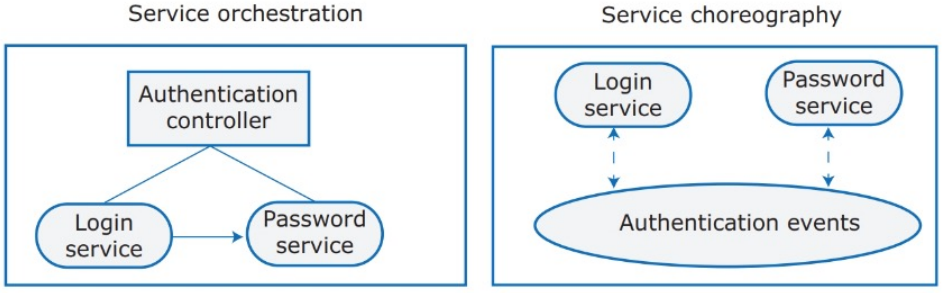
\includegraphics[width=1\textwidth]{images/Microservices/orchestration-vs-choreography.PNG}
    \caption{Example of orchestration and choreography}
    \label{fig:orchestration-vs-choreography}
\end{figure} 

From Figure \ref{fig:orchestration-vs-choreography}, we can see that in the case of service orchestration, there's an explicit controller orchestrating the system (in the example, the controller is named Authentication controller), while in the case of service choreography, an event-based synchronization is used (in the example, a Publish \& Subscribe mechanism named Authentication events). The latter allows for the absence of an additional explicit controller (to avoid single points of failure), but it is harder to debug and recover in case of failure. \\

A good practice is to always start with orchestration (easier to design) and switch to choreography only if the product is inflexible or hard to update.

\newpage

\subsection{Failure management}

Something will go wrong, unavoidably (e.g., a service offers a functionality \(F\) by invoking two other services, each available 99\% of the time and independent of one another. \(F\) will probably be NOT available for around 30 minutes each day). It's important, especially in distributed environments, to have some kind of \textbf{failure management} in case of failure: services must be designed to cope with failures. \\
\newline\noindent
There are mainly three types of failures:
\begin{itemize}
    \item \textbf{Internal service failure}: These are conditions that are detected by the service and can be reported to the service requester in an error message. An example of this type of failure is a service that takes a URL as input and discovers that it is an invalid link.
    \item \textbf{External service failure}: These failures have an external cause that affects the availability of a service. A failure may cause the service to become unresponsive, and actions have to be taken to restart the service.
    \item \textbf{Service performance failure}: The performance of the service degrades to an unacceptable level. This may be due to a heavy load or an internal problem with the service. External service monitoring can be used to detect performance failures and unresponsive services.
\end{itemize}

One of the most typical solutions used for microservices is \textbf{circuit breakers}: they are design patterns that create resilient microservices by limiting the impact of service failures and latencies. The idea is that (take Figure \ref{fig:circuit-breaker} as a reference) an additional component (the circuit breaker) is added between the service client and the remote service (supplier). This additional component takes a request from the client, forwards it to the remote service, and then starts an internal timer. In the case that the remote service works fine, then the additional component receives the answer from the remote service and forwards it to the service client. If the timer triggers a timeout (either because the remote service failed or was too slow), then the circuit breaker tells the client that the remote service failed (avoiding the clients getting stuck waiting for the remote service response). In case of multiple failures, the circuit breaker \textit{trips}, and for the duration of a timeout period, all attempts to invoke the remote service will fail immediately. After the timeout expires, the circuit breaker allows a limited number of test requests to pass through. If those requests succeed, the circuit breaker resumes normal operation. Otherwise, the timeout period begins again.\\

An interesting example of a circuit breaker is implemented by \textit{Spotify}: the search service sometimes fails (since the service has to search through a huge index of songs), so Spotify quickly refreshes the page and uses the time users take to write the name of the song as a cooldown period. Error messages do not pop up.

\begin{figure} [H]
    \centering
    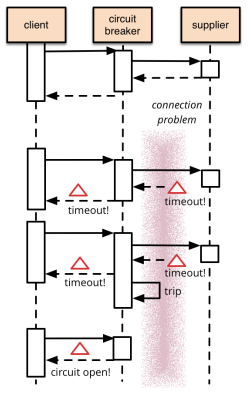
\includegraphics[width=0.4\textwidth]{images/Microservices/circuit-breaker.PNG}
    \caption{Example of a circuit breaker sequence diagram}
    \label{fig:circuit-breaker}
\end{figure} 

There are many ways to test failure management. One interesting way implemented by Netflix is \textit{Chaos Monkey}\footnote{\url{https://netflix.github.io/chaosmonkey/}} (which comes from chaos engineering), a tool that randomly terminates VM instances and containers running inside a production environment. This type of testing is done during the production phase; that's why this is called a \textit{bravely} conducted test.

\section{RESTful services}

Microservices are \textbf{RESTful services}. REpresentational State Transfer (REST) has four main principles:

\begin{itemize}
    \item \textbf{Resource identification through URIs}: the service exposes a set of resources, where each resource is identified by a URI\footnote{Uniform Resource Identifier (URI) is a character sequence that identifies a logical (abstract) or physical resource}.
    \item \textbf{Uniform interface}: clients invoke HTTP methods to create/read/update/delete resources (with POST and PUT to create and update the state of a resource, DELETE to delete a resource, and GET to retrieve the current state of a resource).
    \item \textbf{Self-descriptive messages}: Requests contain enough contextual information to process messages, since information can be accessed in various formats (e.g., HTML, XML, JSON, plain text, PDF, JPEG, etc.). This is why resources are decoupled from their representation.
    \item \textbf{Stateless interactions through hyperlinks}: every interaction with a resource is stateless, which means that servers contain no client state, and any session state is held on the client. Stateless interactions rely on the concept of explicit state transfer.
\end{itemize}

There are many other things to say about REST, but they have already been covered during the bachelor's degree.

\section{Service deployment}

For the past 70 years, for each software project, a group of developers managed the entire life cycle based on project-based software engineering (requirement definition, specifications, prototype, testing, integration, quality of experience, and so on). Once the software is completed, the operations team (which did not participate in the development) puts the software into production (possibly in a different environment from where the software was developed) and then responds to customer problems.

\begin{figure} [H]
    \centering
    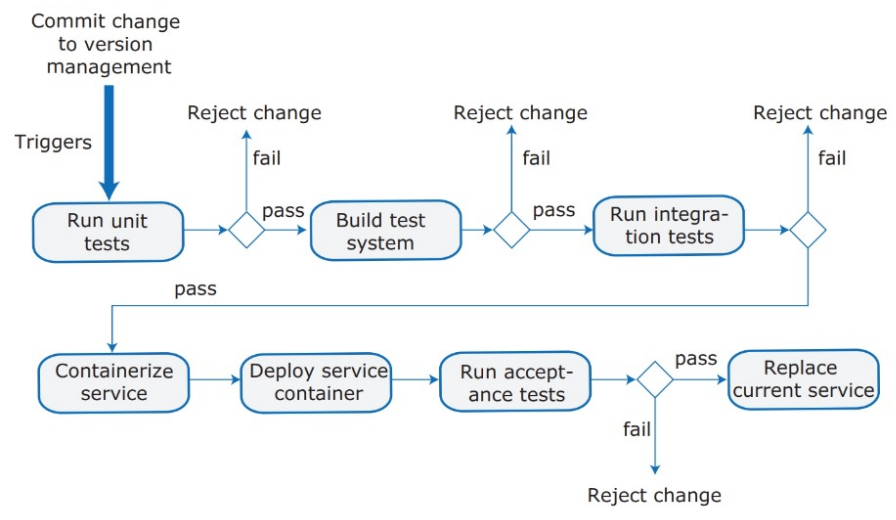
\includegraphics[width=0.93\textwidth]{images/Microservices/DevOps.PNG}
    \caption{Continuous Deployment pipeline}
    \label{fig:DevOps}
\end{figure} 

The new era of software engineering is DevOps (a portmanteau of “development” and “operations”): the same team is responsible for service development, deployment, and management. From Figure \ref{fig:DevOps}, we can see the pipeline that software developers use when there's a commit request: the pipeline starts unit tests, makes the build, runs the integration, containerizes, deploys, runs the tests, and if everything goes right, replaces the current service with the new commit.

\subsection{Monitoring}

Testing cannot prevent 100\% of unanticipated problems, which means that there is a need to monitor the deployed services. If you do not monitor microservices, you cannot know the state of the services, but excessive monitoring can lead to performance degradation. As with many things in microservices, a trade-off must be found.

\begin{figure} [H]
    \centering
    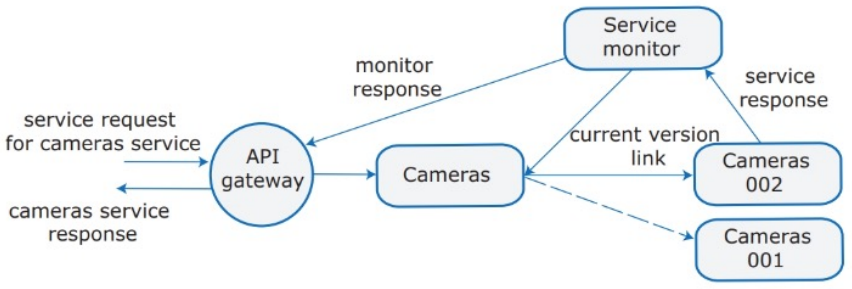
\includegraphics[width=0.88\textwidth]{images/Microservices/Monitor-example.PNG}
    \caption{Monitoring example}
    \label{fig:Monitor-example}
\end{figure} 

The example shown in Figure \ref{fig:Monitor-example} illustrates that it's also possible to increase reliability with monitoring: when a new version of a service is introduced, it's possible to maintain the old version while changing the “current version link” to point to the new service. If monitoring detects a problem with the new version of the “Cameras 002” service, it switches the “current version link” back to version 001 of the Cameras service.


\section{Architectural smells}

An \textbf{architectural smell} is a commonly used architectural decision that negatively impacts system lifecycle qualities. Once the microservice principles are defined, how can architectural \textcolor{red}{smells} affecting the design \textcolor{blue}{principles} of microservices be detected and then resolved via \textcolor{green}{refactoring}?

This section will show, based on a \textit{multivocal review} (which uses both scientific articles and technical websites), the most recognized \textit{architectural smells} for microservices and the architectural \textit{refactorings} to resolve them. \newline The \textbf{design principles} that will be taken into consideration are:

\begin{itemize}
    \item \textcolor{blue}{Independent deployability}: the microservices forming an application should be independently deployable.
    \item \textcolor{blue}{Horizontal scalability}: the microservices forming an application should be horizontally scalable (which means the possibility of adding/removing replicas of individual microservices).
    \item \textcolor{blue}{Isolation of failures}: failures should be isolated (avoiding the cascade effect).
    \item \textcolor{blue}{Decentralization}: decentralization should occur in all aspects of microservice-based applications, from data management to governance.
\end{itemize}

\subsection{Smells and refactoring}

All the \textcolor{red}{architectural smells} will be categorized based on the \textcolor{blue}{design principle} they violate. For each smell, some \textcolor{green}{refactorings} will be presented to resolve them.

\subsubsection{Independent deployability}

One \textit{architectural smell} for \textcolor{blue}{independent deployability} is \textcolor{red}{multiple services in one container} (because ideally we want to have one container per microservice). It is possible to insert some microservices that interact a lot inside the same container, but this can lead to various problems. The solution for this smell is to \textcolor{green}{package each service in a separate container}.

\subsubsection{Horizontal scalability}

One common \textit{architectural smell} for \textcolor{blue}{horizontal scalability} is \textcolor{red}{endpoint-based service interaction}. This is a smell because, if there is an interaction with a specific service instance (as shown in Figure \ref{fig:end-point-img1}), adding more replicas of the service won't scale the application since the interaction is made with only one of the replicas. Some \textit{refactorings} for the described \textit{smell} are to \textcolor{green}{add a service discovery} that will indicate to the requester which replica they must use (applied in 55\% of cases), \textcolor{green}{add a message router} that will redirect the request to one of the replicas (e.g., load balancer, applied in 31\% of cases), or \textcolor{green}{add a message broker} that will collect the requests, which are then processed by the replicas (e.g., message queue, applied in 14\% of cases). The reason that the message broker is the least used is that the code of the microservice has to be modified.

\begin{figure} [H]
    \centering
    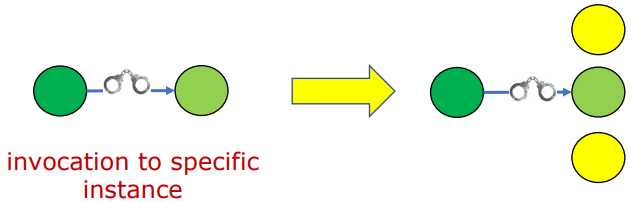
\includegraphics[width=0.65\textwidth]{images/Microservices/end-point-img1.PNG}
    \caption{Endpoint-based service interaction}
    \label{fig:end-point-img1}
\end{figure} 

Another \textit{architectural smell} is the \textcolor{red}{absence of an API gateway}, because clients can invoke the services directly (which is similar to the endpoint-based service interaction smell). The solution is simply to \textcolor{green}{add an API gateway}, as it not only resolves the smell but can also be useful for authentication, throttling, and so on.

\newpage 

\subsubsection{Isolation of failures}

One \textit{architectural smell} for \textcolor{blue}{isolation of failures} is \textcolor{red}{wobbly service interaction}: the interaction of m1 with m2 is \textit{wobbly} when a failure of m2 can trigger a failure of m1. Some \textit{refactorings} for the described \textit{smell} are to \textcolor{green}{add a circuit breaker} (applied in 42\% of cases), \textcolor{green}{use timeouts} (applied in 22\% of cases), \textcolor{green}{add a bulkhead} (applied in 20\% of cases), or \textcolor{green}{add a message broker} (applied in 16\% of cases).

\subsubsection{Decentralization}

One common \textit{architectural smell} for \textcolor{blue}{decentralization} is \textcolor{red}{shared persistence}. Three proposed solutions (which are better described in Figure \ref{fig:shared_persistence}) are \textcolor{green}{split database} (applied in 50\% of cases), \textcolor{green}{add a data manager} that acts as a gateway between the services and the database (applied in 22\% of cases), or \textcolor{green}{merge services} (applied in 9\% of cases).

\begin{figure} [H]
    \centering
    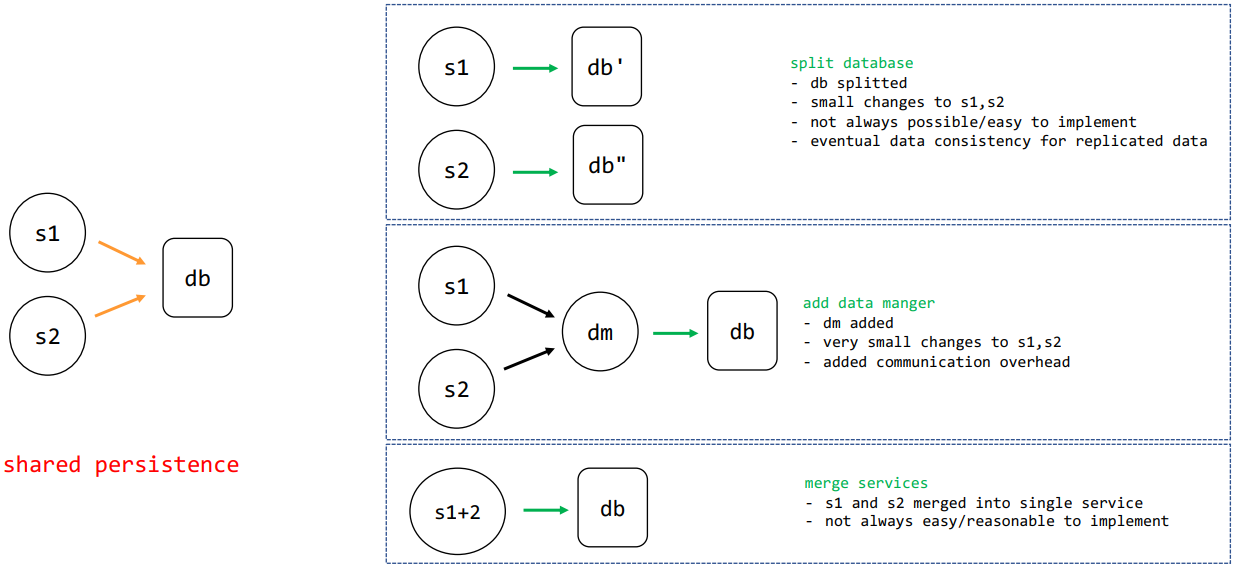
\includegraphics[width=1\textwidth]{images/Microservices/shared_persistence.PNG}
    \caption{Solutions for shared persistence}
    \label{fig:shared_persistence}
\end{figure} 

The last \textit{architectural smell} is the \textcolor{red}{single-layer teams}, which goes against the idea of Agile. The solution is simply to \textcolor{green}{split teams by service}.

\subsection{A toolchain for microservices}

Now that we know about these \textit{architectural smells}, we want to identify and solve them. The first step is to create a graphical representation of our architecture, as shown in Figure \ref{fig:modelling-application-architecture}. This is done to better understand the structure of the application.

These models also allow for \textit{team-based views}, as each service is developed by a different team. This is particularly useful in cases where there may be smells between two or more microservices managed by different teams. It enables teams to detect these smells and make necessary arrangements to address and fix them.

\begin{figure} [H]
    \centering
    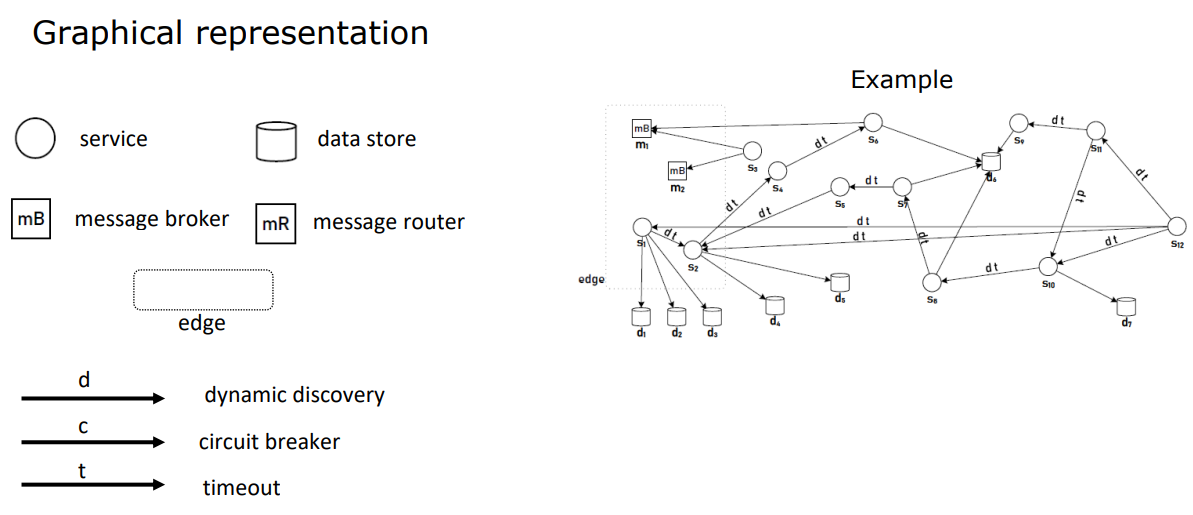
\includegraphics[width=1\textwidth]{images/Microservices/modelling-application-architecture.PNG}
    \caption{Modelling application architecture}
    \label{fig:modelling-application-architecture}
\end{figure} 

There are tools that take these models as input and provide, as output, the smells present in the application. One developed by the University of Pisa is MicroFreshner\footnote{\url{https://github.com/di-unipi-socc/microFreshener}}. It may be hard to obtain the modeled application architecture in the case of a large system, so tools have been created (such as MicroMiner and MicroTOM) to obtain those models by providing the K8s manifest and performing some dynamic analysis of the running application (noting that container orchestration does change application behavior). From Figure \ref{fig:toolchain}, we can see the toolchain used to fix microservices smells.

\begin{figure} [H]
    \centering
    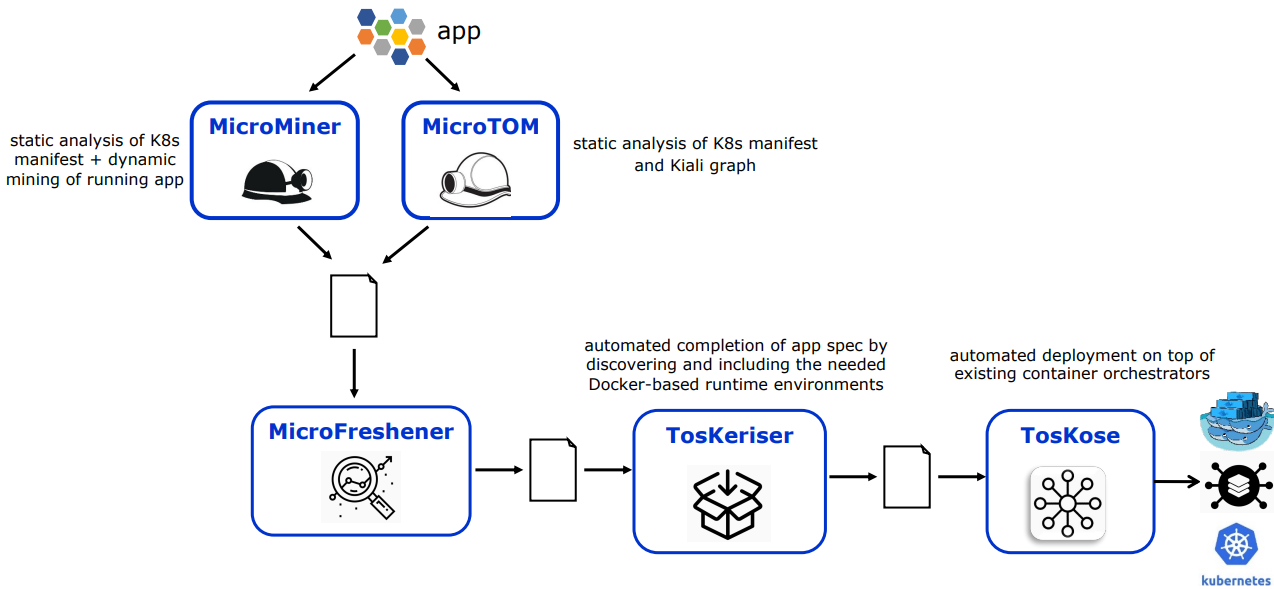
\includegraphics[width=1\textwidth]{images/Microservices/toolchain.PNG}
    \caption{Toolchain for microservices}
    \label{fig:toolchain}
\end{figure} 

Once the smells have been analyzed and some fixes have been made inside MicroFreshner, it is possible to take the result of MicroFreshner and automatically deploy the fixed architecture on top of the existing container orchestrator.

